\documentclass{article}

% Language setting
% Replace `english' with e.g. `spanish' to change the document language
\usepackage[english]{babel}
\usepackage{float}

% Set page size and margins
% Replace `letterpaper' with `a4paper' for UK/EU standard size
\usepackage[letterpaper,top=2cm,bottom=2cm,left=3cm,right=3cm,marginparwidth=1.75cm]{geometry}

% Useful packages
\usepackage{amsmath}
\usepackage{float}
\usepackage{graphicx}
\usepackage[colorlinks=true, allcolors=blue]{hyperref}

\title{Session 11 project}
\author {
      Gkloumpos Nikolaos,
      Malthe H. Boelskift,
      Louis Ildal,
      Guillermo V. Gutierrez-Bea,
}

\begin{document}
\maketitle

\text {
      Group: 203
}

\section{Discussions of results} 

We have tried to change the hyper-parameters for better results, and played around with it. 

The Iteration parameter obviously determines how many iterations of the algorithm will be performed. 
More iterations can potentially lead to better noise reduction but may also increase the computational time.
So it is not so ideal to have this too high.

The wdiff parameter  controls the relative weight of the difference component in the energy function. 
Adjusting this value can affect how strongly the algorithm penalizes differences between neighboring pixels. 
A lower value might result in smoother images but could also lead to under-smoothing, depending on other parameters.

The maxdiff parameter sets an upper limit on the differences between neighboring pixel values. 
A higher maxdiff allows for greater variation between neighboring pixels before a penalty is applied. 
Lowering this value might encourage smoother reconstructions, if correlated fairly with the wdiff parameter.

We can observe that the algorithm has smoothed the noise, making the image more clear again. 
Speficially surfaces of slowly-varying intensity, e.g., the floor and window is well restored. 
However, areas with rapidly-varying intensities, e.g., motorcycle parts and text, are not as well restored.

\begin{figure}[H]
      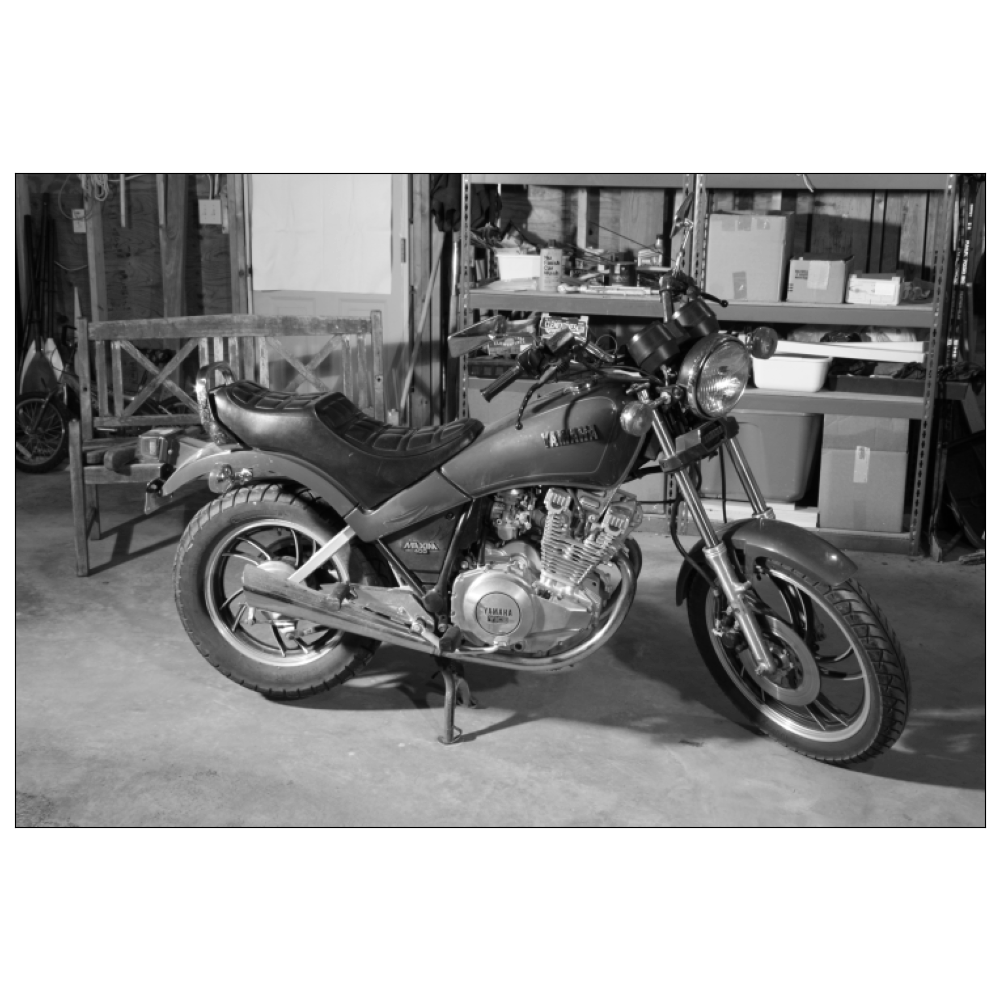
\includegraphics[width=8cm]{assets/Original.png}
      \centering
      \caption{Original Image}
\end{figure}

\begin{figure}[H]
      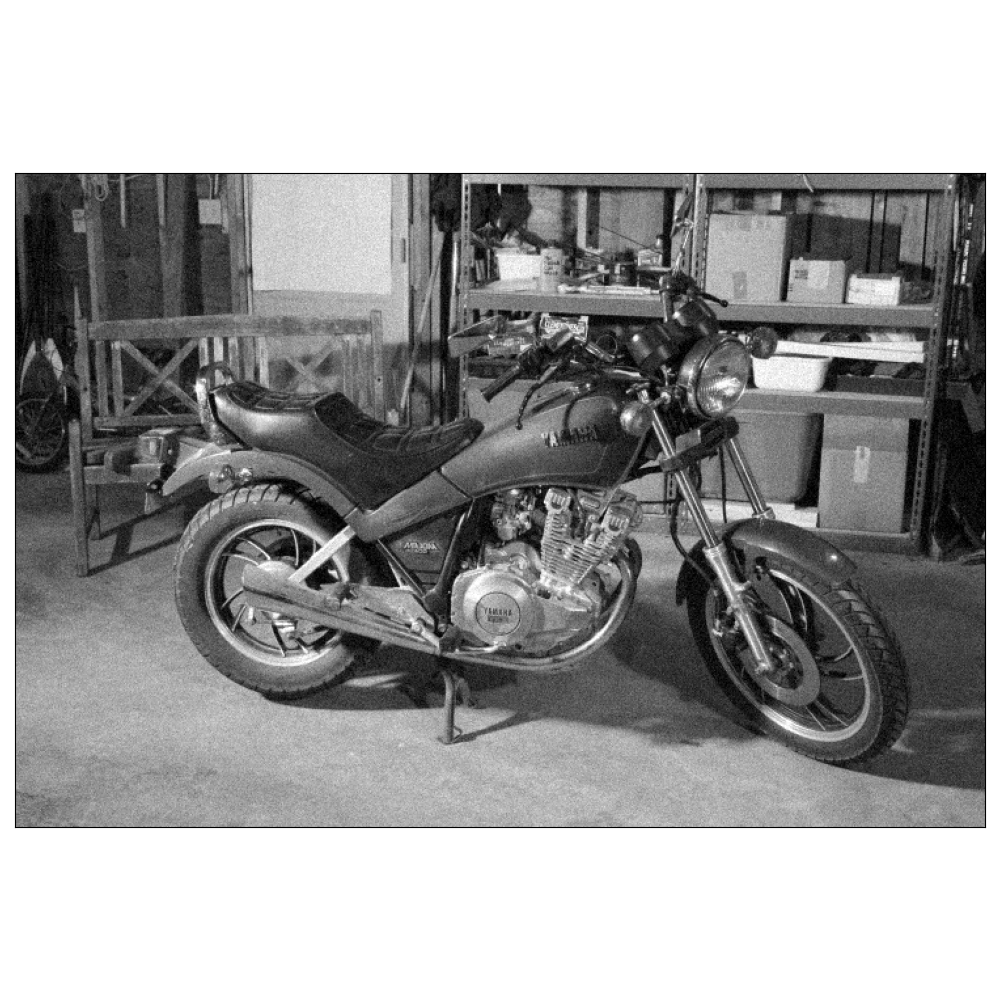
\includegraphics[width=8cm]{assets/Noisy.png}
      \centering
      \caption{Noisy Image}
\end{figure}

\begin{figure}[H]
      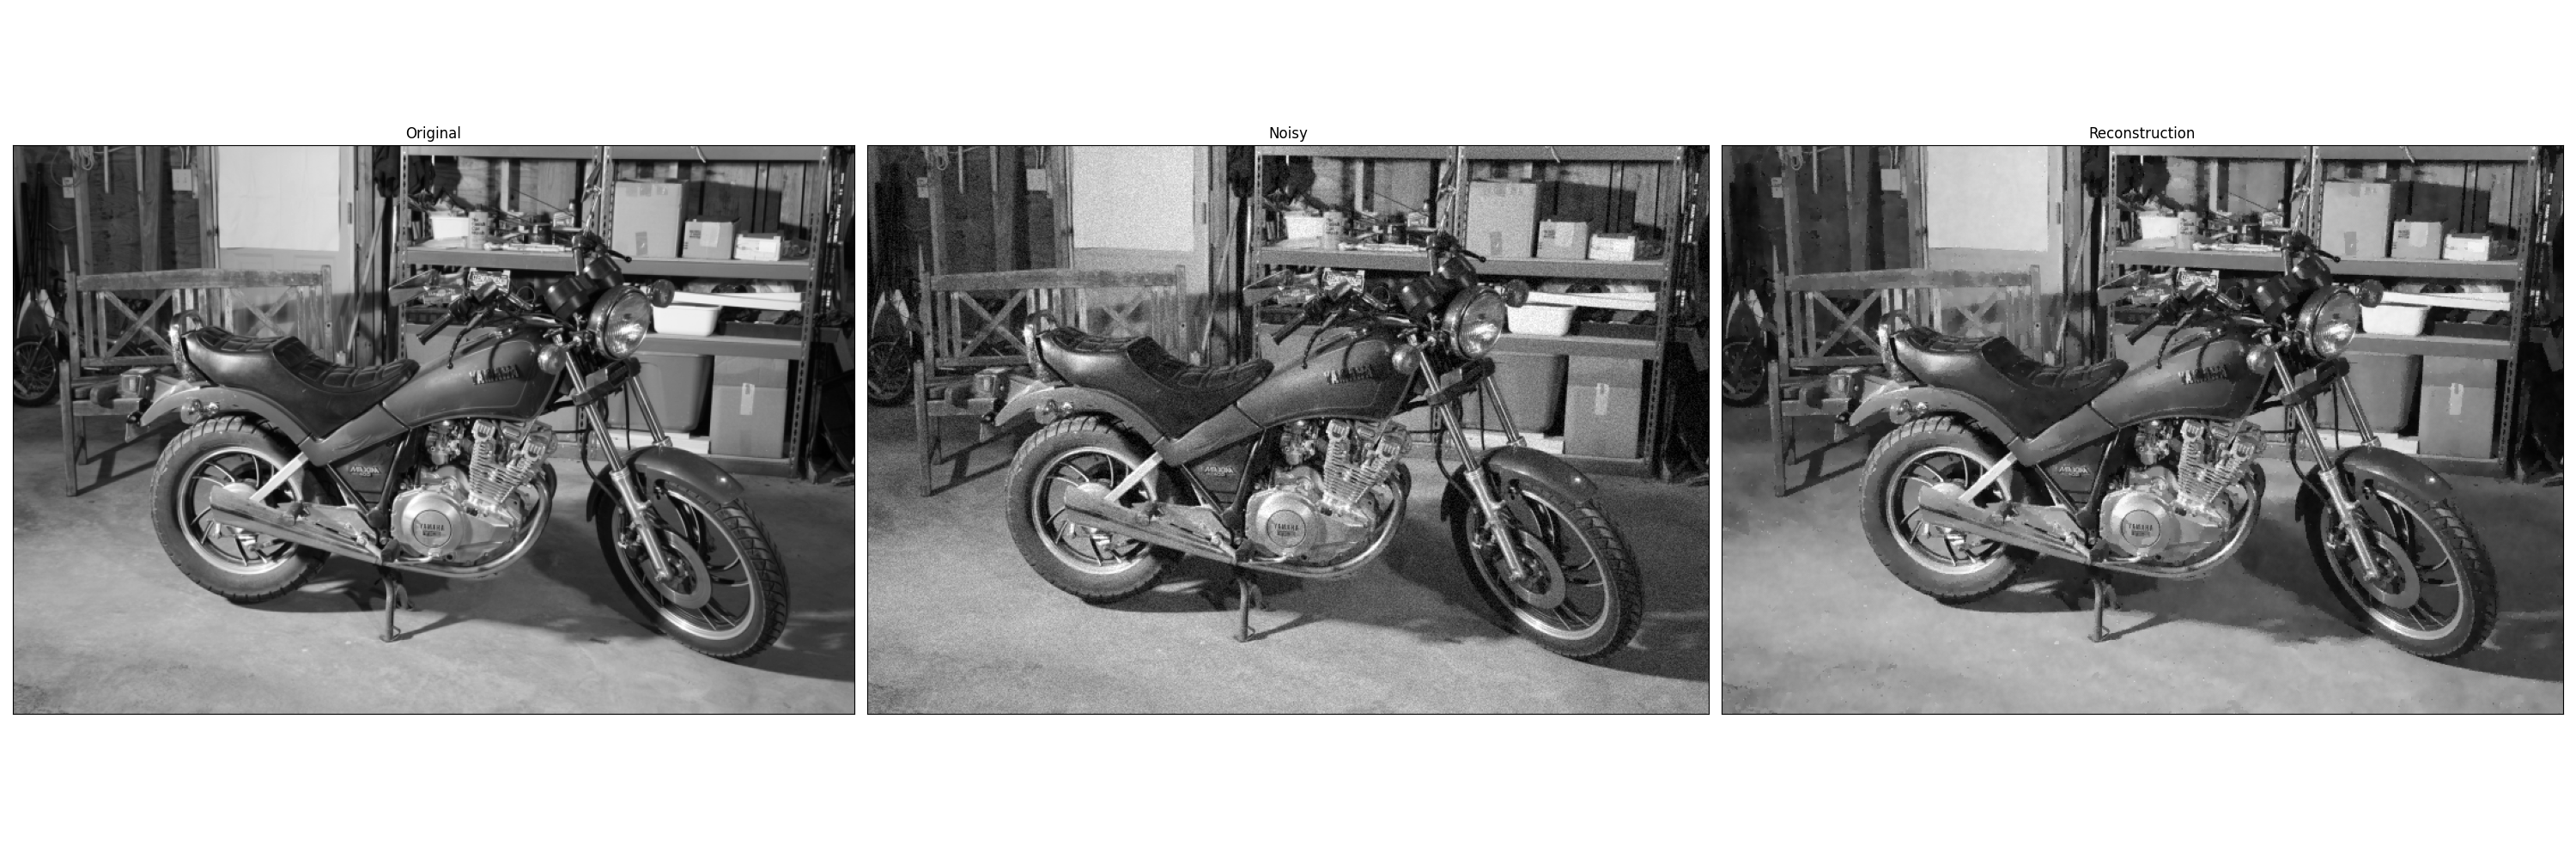
\includegraphics[width=16cm]{assets/FinalComparison.png}
      \centering
      \caption{Final comparison}
\end{figure}

\section {Environment reproduction}
To reproduce the environment used to build the excersise, follow these instructions:

\begin{verbatim}
python3 -m venv env
source env/bin/acivate
pip3 install numpy scikit-learn matplotlib
\end{verbatim}

After the above steps the program can be executed by typing

\begin{verbatim}
python3 `ProgramName.py'
\end{verbatim}

\bibliographystyle{alpha}
\bibliography{sample}

\end{document}